\documentclass{beamer}

\mode<presentation> {
  \usetheme{Warsaw}
  \usecolortheme[rgb={0.37,0.62,0.63}]{structure}

  \setbeamercovered{highly dynamic}
  \usefonttheme{serif}
  \usepackage{ragged2e}
	\justifying
}

\usepackage[spanish]{babel}
\usepackage[utf8]{inputenc}
\usepackage{times}
\usepackage[T1]{fontenc}
\usepackage{amsmath}
\usepackage{amssymb}
\usepackage{verbatim}
\usepackage{hyperref}
\usepackage{xcolor}
\usepackage{booktabs}
\usepackage{tikz}
\usetikzlibrary{arrows.meta,positioning,shapes.geometric,calc}
\usepackage{array}

%%%%%%%%%%%%
\title[35° Simposio Internacional de Estadística]{\textit{\textbf{Nowcasting} del crecimiento económico en Colombia mediante modelos bayesianos de frecuencia mixta}}
%\subtitle{\textit{Evidence from Colombia (2013–2024)}}

\author[Moreno, Olivero y Campo (2026). Nowcasting bayesiano]{Juan Diego Moreno Sánchez \inst{1} \and \and Zeneth Olivero Tapia \inst{2} \\[0.1cm]
\and Jacobo Campo Robledo \inst{1}^{,} \inst{2}}
\institute[Universidad Externado de Colombia -- Universidad Católica de Colombia]
{ 
		\inst{1} Universidad Externado de Colombia
%		\and
%		\inst{2} Universidad Católica de Colombia 
		\and 	
		\inst{2} Universidad Católica de Colombia
}

\date{\footnotesize{Julio 14 de 2026}}

\pgfdeclareimage[height=0.4cm]{logo.jpg}{logo}
\logo{\pgfuseimage{logo.jpg}}

\pgfdeclareimage[height=0.4cm]{logo.jpg}{logo}
\pgfdeclareimage[height=0.4cm]{logouex.jpg}{logouex}
%\logo{\pgfuseimage{logo.jpg}}

\setbeamertemplate{sidebar left}
{
\logo{\pgfuseimage{logouex.jpg}}
\vfill
\rlap{\hskip 0.1cm\insertlogo}
\vskip10pt
}

\beamerdefaultoverlayspecification{<+->}


\begin{document}

\begin{frame}
	\titlepage
\end{frame}

\begin{frame}
	\frametitle{Contenido}
	\tableofcontents[pausesections,pausesubsections]
\end{frame}


\section{Introducción - Problema}

\begin{frame}{Introducción - Problema}
\textcolor[rgb]{0,0,1}{\textbf{El Problema}} 
\begin{itemize}\justifying
	\item El PIB es el indicador más importante para monitorear el ciclo económico, pero en Colombia (como en la mayoría de países) se publica trimestralmente y con rezago (DANE publica ~45 días después del cierre del trimestre). \pause
	\item Entre el cierre de un trimestre y la publicación oficial, los hacedores de política, analistas de mercado y el sector privado deben tomar decisiones sin saber aún qué pasó con la economía. \pause
	\item En contraste, existe un conjunto amplio de indicadores de alta frecuencia (mensual) disponibles casi en tiempo real: ISE, producción manufacturera, ventas del comercio, inflación, tasa de cambio, tasa de política monetaria, precio del petróleo.
\end{itemize}
\end{frame}

\begin{frame}{Introducción - Problema}{}
\begin{itemize}\justifying
	\item El \textit{\textbf{nowcasting}} busca cerrar esa brecha: usar la información mensual disponible para estimar el crecimiento del trimestre antes de que se publique el dato oficial. \pause
	\item Limitación central: desfase de frecuencia y de tiempo entre el PIB (trimestral, rezagado) y los indicadores de actividad (mensuales, casi en tiempo real). \pause
	\item Agregar mecánicamente los datos mensuales a trimestral para "`esperar"' y estimar un VAR trimestral desperdicia información — se pierde la actualización progresiva que ocurre mes a mes dentro de cada trimestre.
\end{itemize}
\end{frame}

\begin{frame}{Introducción - Problema}{}
\begin{itemize}\justifying
	\item Necesidad de un marco que:
	\begin{itemize}
		\item Actualice el pronóstico cada vez que llega un nuevo dato mensual (no solo al cierre del trimestre)
		\item Maneje el ragged edge (distintos calendarios de publicación: el ISE sale antes que la inflación, que sale antes que el PIB, etc.) sin forzar a todas las series al mismo calendario
		\item Sea manejable en un país con series relativamente cortas y alta volatilidad macroeconómica (commodities, tasa de cambio)
	\end{itemize}
	\item Esto motiva un MF-BVAR (Bayesian Mixed-Frequency VAR), que trata al PIB como una variable latente mensual parcialmente observada.
\end{itemize}
\end{frame}

\begin{frame}{Introducción - Problema}{¿Por qué un enfoque bayesiano?}
\begin{itemize}\justifying
	\item Un VAR mensual con varias variables y varios rezagos tiene muchos parámetros en relación con el número de observaciones disponibles (\textit{sobreparametrización}) — estimarlo por MV/OLS sin restricciones produce coeficientes muy inestables y sobreajuste. \pause
	\item El enfoque bayesiano permite introducir \textit{priors} de contracción (\textit{shrinkage}), el prior de Minnesota (Litterman, 1986):
	
	\begin{itemize}\justifying
		\item Regulariza los coeficientes hacia una estructura parsimoniosa (ej. paseo aleatorio) sin eliminar variables arbitrariamente
		\item Permite incluir más variables e indicadores de los que un VAR clásico toleraría con series relativamente cortas,
		\item Mejora la precisión fuera de muestra frente a alternativas no restringidas (Bańbura, Giannone y Reichlin (2010)).
	\end{itemize}

\end{itemize}
\end{frame}

\begin{frame}{Introducción - Problema}{¿Por qué un enfoque bayesiano?}
\begin{itemize}\justifying
	\item Además, el marco bayesiano entrega una distribución \textit{posterior} completa del pronóstico (no solo un punto), lo que permite cuantificar la incertidumbre alrededor del \textbf{nowcast} — información valiosa para el análisis de riesgo y la comunicación de política. \pause
	\item El tratamiento de frecuencia mixta (\textit{variable trimestral parcialmente observada}) se resuelve de forma natural dentro de una representación de espacio de estados (\textbf{filtro de Kalman}), que es el marco estándar para inferencia bayesiana en modelos dinámicos.
\end{itemize}
\end{frame}

\begin{frame}{Introducción - Problema}
\begin{block}{Objetivo general}\justifying
Proponer y estimar un modelo de \textit{nowcasting} del crecimiento económico de Colombia mediante un Bayesian Mixed-Frequency VAR (MF-BVAR), que permita actualizar el pronóstico del PIB trimestral a partir de indicadores mensuales de actividad real, precios, condiciones financieras y sector externo.
\end{block}
\end{frame}



\section{Marco Teórico y Revisión de Bibliografía}

\begin{frame}{Marco Teórico y Revisión de Bibliografía}{}
\begin{itemize}\justifying
	\item \textcolor[rgb]{0,0.58,0}{Giannone, Reichlin y Small (2008)}: definen el nowcasting como la actualización continua del pronóstico del trimestre corriente conforme llega nueva información.
	\item \textcolor[rgb]{0.92,0.5,0.4}{Mariano y Murasawa (2003)}: proponen el índice coincidente basado en series mensuales y trimestrales — base de la identidad de agregación en un MF-BVAR.
	\item \textcolor[rgb]{0.92,0.5,0.4}{Kuzin, Marcellino y Schumacher (2011)}: comparan MIDAS vs. VAR de frecuencia mixta para nowcasting del PIB de la eurozona.
	\item \textcolor[rgb]{0.92,0.5,0.4}{Carriero, Clark y Marcellino (2015)}: extienden el MF-BVAR con volatilidad estocástica para pronóstico en tiempo real.
\end{itemize}
\end{frame}

\begin{frame}{Marco Teórico y Revisión de Bibliografía}{}
\begin{itemize}\justifying
	\item \textcolor[rgb]{0,0,1}{Litterman (1986)}: origen del \textit{prior} de Minnesota.
	\item \textcolor[rgb]{0,0,1}{Banbura, Giannone y Reichlin (2010)}: BVAR grandes con contracción — muestran que permite incluir muchas variables sin perder precisión predictiva.
	\item \textcolor[rgb]{0.29,0,0.51}{Schorfheide y Song (2015)}: desarrollan el marco de pronóstico en tiempo real que combina variables mensuales y trimestrales en una estructura VAR de frecuencia mixta.
\end{itemize}
\end{frame}


\section{Datos y Metodología}

\subsection{Datos}

\begin{frame}{Datos}{}\justifying
Se construye un sistema de frecuencia mixta con \textbf{9 variables} para Colombia, combinando una serie trimestral objetivo y ocho indicadores mensuales de actividad real, precios, condiciones monetarias y sector externo. \pause

\begin{table}[h]
\centering
\tiny
\begin{tabular}{llll}
\toprule
\textbf{Variable} & \textbf{Frecuencia} & \textbf{Fuente} & \textbf{Rol} \\
\midrule
PIB real & Trimestral & DANE & Variable objetivo \\
ISE & Mensual & DANE & Actividad económica agregada \\
IPI (Producción industrial) & Mensual & DANE & Sector manufacturero \\
Tasa de desempleo & Mensual & DANE & Mercado laboral \\
Inflación (IPC) & Mensual & DANE & Precios \\
TRM & Mensual & Banco de la República & Sector externo / financiero \\
Tasa de política monetaria & Mensual & Banco de la República & Condiciones monetarias \\
Petróleo (Brent) & Mensual & Mercados internacionales & Choque externo (términos de intercambio) \\
IEC & Mensual & Fedesarrollo & Expectativas \\
\bottomrule
\end{tabular}
\end{table}
\end{frame}

\begin{frame}{Datos}{Muestra y Transformaciones}\justifying
\begin{itemize}\justifying
    \item \textbf{Muestra histórica}: 2014--2025 (144 meses, 48 trimestres).
    \item \textbf{Muestra de nowcasting}: 2021--2025 (submuestra reciente, usada para el ejercicio de pronóstico en tiempo real).
    \item Todas las series mensuales se emplean desestacionalizadas.
    \item Las variables se modelan \textbf{en niveles}; la no estacionariedad se controla directamente a través del \textit{prior} de Minnesota, que impone la hipótesis de \textit{random walk} sobre el primer rezago propio de cada variable.
\end{itemize}
\end{frame}


\subsection{Metodología}

\begin{frame}{Metodología}{Panorama General}\justifying
El modelo se estima en tres etapas: \pause
\begin{enumerate}\justifying
    \item \textbf{Especificación}: VAR mensual en forma de espacio de estados, con el PIB trimestral como variable parcialmente observada (Schorfheide y Song, 2015). \pause
    \item \textbf{Estimación bayesiana}: muestreador de Gibbs, combinando simulación de estados (Carter-Kohn, 1994) y actualización de parámetros bajo \textit{prior} de Minnesota. \pause
    \item \textbf{Proyección}: densidad predictiva conjunta del PIB mensual latente, agregada de forma consistente al horizonte trimestral de interés.
\end{enumerate}
\end{frame}

\begin{frame}{Metodología}{Formulación del Modelo de Espacio de Estados MF-VAR}\justifying
Sea $x_t = [x_{m,t}', x_{q,t}']'$ un vector $n \times 1$ de variables macroeconómicas. La ecuación de transición mensual en representación compañera $np \times 1$ es: \pause
\[
Z_t = F(\Phi) Z_{t-1} + F_c(\Phi) + V_t, \quad V_t \sim \text{i.i.d. } N(0, \Omega(\Sigma))
\] \pause
Donde la matriz compañera $F(\Phi)$ y la covarianza singular $\Omega(\Sigma)$ se definen como: \pause
\[
F(\Phi) = \begin{bmatrix} \Phi_1 & \Phi_2 & \dots & \Phi_p \\ I_{n(p-1)} & & 0_{n(p-1) \times n} \end{bmatrix}, \quad \Omega(\Sigma) = \begin{bmatrix} \Sigma & 0 \\ 0 & 0 \end{bmatrix}
\]
\end{frame}

\begin{frame}{Metodología}{Formulación del Modelo de Espacio de Estados MF-VAR}\justifying
La ecuación de medición en presencia de datos faltantes temporales \pause
\[
Y_t^{obs} = M_t \Lambda Z_t
\] \pause
donde $\Lambda$ es la matriz de agregación temporal \textit{log-lineal} y $M_t$ es la matriz de selección variante que depura las celdas vacías (\texttt{NA}) en cada mes $t$, solucionando estructuralmente el problema del \textbf{\textit{ragged edge}} (borde irregular) en la publicación de datos. \\ \pause
En el horizonte $T+1, \dots, T+H$, el PIB mensual latente $x_{q, T+h}^*$ se proyecta mediante la densidad predictiva conjunta:  \pause \small{
\[
p(Z_{T+1:T+H} \mid Y_{1:T}^{obs}) = \int p(Z_{T+1:T+H} \mid Z_T, \Phi, \Sigma) p(\Phi, \Sigma \mid Y_{1:T}^{obs}, Z_{1:T}) \, d(\Phi, \Sigma)
\]}
\end{frame}

\begin{frame}{Metodología}{Distribución Predictiva Posterior del Estado Latente}\justifying
El muestreador de Gibbs simula esta distribución iterando sobre: \pause
\begin{enumerate}\justifying
    \item \textbf{Simulación de Estados (Carter-Kohn, 1994)}: Sorteo de la trayectoria $Z_{1:T}$ condicionado a los parámetros del modelo: \pause
    \[
    p(Z_{1:T} \mid Y_{1:T}^{obs}, \Phi, \Sigma) \propto p(Z_0) \prod_{t=1}^T p(Y_t^{obs} \mid Z_t) p(Z_t \mid Z_{t-1}, \Phi, \Sigma)
    \]
    \item \textbf{Paso de Parámetros}: Sorteo de $(\Phi, \Sigma)$ condicionado al vector de estados simulado desde la posterior normal-Wishart inversa: \pause
    \[
    p(\Phi, \Sigma \mid Y_{1:T}^{obs}, Z_{1:T}) \sim MNIW(\bar{\Phi}, \bar{\Psi}, \bar{\Sigma}, \bar{\nu})
    \]
\end{enumerate}
\end{frame}


\begin{frame}{Metodología}{Proyección Dinámica y Agregación Consistente}\justifying
El PIB mensual latente $PIB_{M,t}^*$ es una variable de estado estimada por la estructura dinámica del sistema, no un promedio de la serie trimestral. \pause
\begin{itemize}\justifying
    \item Como el PIB es una variable de flujo en niveles, la agregación trimestral opera estrictamente como una \textbf{restricción de medición} aditiva en el Filtro de Kalman: \pause
    \[
    PIB_{Q, t} = PIB_{M, t}^* + PIB_{M, t-1}^* + PIB_{M, t-2}^*
		\]
    \item Así, el pronóstico para Q1-2026 se calcula agregando los meses latentes proyectados de Enero, Febrero y Marzo de 2026:
\end{itemize}
\end{frame}

\begin{frame}{Metodología}{Calibración y Diagnósticos de Convergencia MCMC}
\begin{itemize}\justifying
    \item \textbf{Prior de Minnesota}: $\lambda_1 = 0.09$. Controla la contracción de los coeficientes hacia la hipótesis de \textit{random walk} en cada variable.
    \item \textbf{Simulaciones}: 20{,}000 (\textit{draws}), 10{,}000 calentamiento (\textit{burn-in}).
    \item \textbf{Especificación de rezagos}: $p=6$ en la muestra histórica completa; $p=4$ en la submuestra de nowcasting (2021--2025), para evitar singularidad en la matriz de covarianza del prior.
    \item \textbf{Tamaño de muestra efectivo (ESS)}:
    \begin{itemize}\justifying
        \item Muestra histórica ($p=6$): ESS $= 13{,}775.04$
        \item Muestra de nowcasting ($p=4$): ESS $= 9{,}797.47$
    \end{itemize}
    \item Un ESS alto (\textit{relativo}) indica baja autocorrelación en la cadena y buena mezcla del muestreador de Gibbs (convergencia adecuada).
\end{itemize}
\end{frame}


\section{Estimaciones y Resultados}

\begin{frame}{Estimaciones y Resultados}{Evaluación Puntual del Nowcast}\justifying
Comparación entre el dato observado de DANE y la mediana posterior del MF-BVAR para el trimestre evaluado: \\[0.2cm] \pause
\begin{table}[h]
\centering
\tiny
\begin{tabular}{lcccc}
\toprule
\textbf{Métrica / Fecha} & \textbf{Dato Real DANE} & \textbf{Mediana BVAR} & \textbf{Bandas 95\%} & \textbf{Error \%} \\
\midrule
PIB real (niveles) & 258,780.7 & \textbf{257,736.6} & [252,880.7 \text{ a } 262,695.5] & 0.40\% \\
Crec. Inter (Q) & +0.58\% & \textbf{0.18\%} & [-1.70\% \text{ a } 2.11\%] & --- \\
Crec. Inter (Y) & +2.17\% & \textbf{1.76\%} & [-0.16\% \text{ a } 3.72\%] & --- \\
\bottomrule
\end{tabular}
\end{table} \\[0.2cm] \pause
El error absoluto en niveles es de solo \textbf{0.40\%}, y el dato observado cae dentro del intervalo de credibilidad al 95\% en ambas métricas de crecimiento.
\end{frame}

\begin{frame}{Estimaciones y Resultados}{Trayectoria del Nowcast: Observado vs. Estimado}
\begin{center}
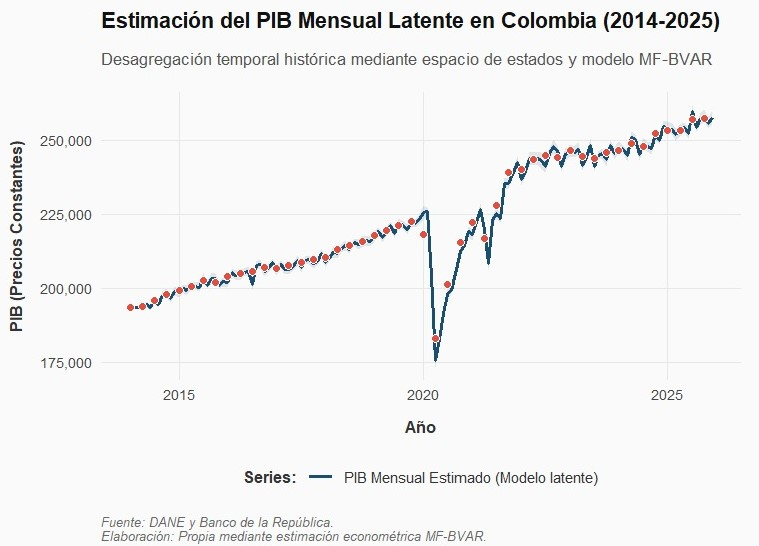
\includegraphics[scale=0.4]{Grafica1.jpeg}
\end{center}
\end{frame}

\begin{frame}{Estimaciones y Resultados}{Trayectoria del Nowcast: Observado vs. Estimado}
\begin{center}
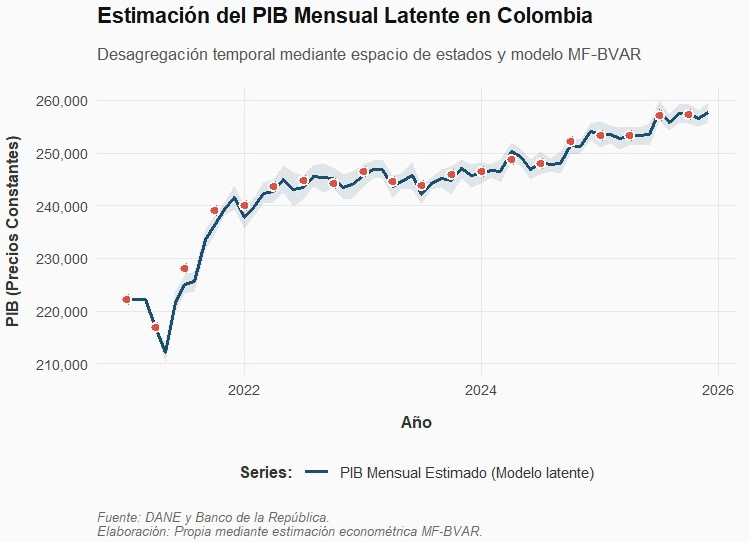
\includegraphics[scale=0.4]{Grafica2.jpeg}
\end{center}
\end{frame}

\begin{frame}{Estimaciones y Resultados}{Pronóstico 2026-Q1}
\begin{center}
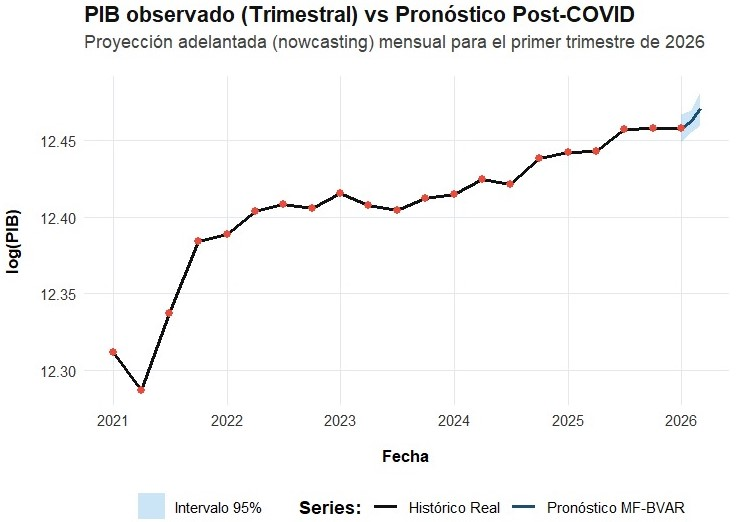
\includegraphics[scale=0.4]{Grafica3.jpeg}
\end{center}
\end{frame}



\section{Consideraciones finales}

%\begin{frame}{Consideraciones finales}{}\justifying
%\begin{block}{ }\justifying

%\end{block}
%\pause
%\begin{itemize}\justifying
%	\item 
%	\item 
%\end{itemize}
%\end{frame}

\begin{frame}{Consideraciones finales}{}
\begin{itemize}\justifying
    \item El MF-BVAR permite generar \textbf{nowcasts mensuales del PIB colombiano} explotando la información disponible antes de la publicación oficial trimestral del DANE, sin sacrificar la coherencia estadística entre frecuencias. \pause
    \item El tratamiento del PIB como \textbf{variable de estado latente} --- y no como un dato interpolado mecánicamente --- permite que la agregación trimestral opere como una restricción de medición exacta dentro del filtro de Kalman. 
\end{itemize}
\end{frame}

\begin{frame}{Consideraciones finales}{}
\begin{itemize}\justifying
    \item La evaluación puntual mostró un error absoluto de solo \textbf{0.40\%} en niveles, con el dato observado cayendo dentro de las bandas de credibilidad al 95\% tanto en crecimiento trimestral como anual. \pause
    \item El enfoque bayesiano (prior de Minnesota + MNIW) resuelve el problema de sobreparametrización inherente a un VAR mensual con múltiples variables y rezagos, permitiendo estimar el sistema incluso con series relativamente cortas.
\end{itemize}
\end{frame}

\begin{frame}{}\justifying
\begin{block}{}
\begin{center}
\huge{\textbf{MUCHAS GRACIAS...!}}
\end{center}
\end{block}
\end{frame}

\end{document}
